\documentclass{article}
\usepackage[a4paper, margin=2.5cm]{geometry}
\usepackage{amsmath}
\usepackage{caption}
\usepackage{placeins}
\usepackage{graphicx}
\usepackage{subcaption}
\usepackage{setspace}
\usepackage{float}

%\usepackage[active,tightpage]{preview}
\usepackage{natbib}
\bibpunct{(}{)}{,}{a}{}{;} 
\usepackage{url}
\usepackage{nth}
\usepackage{authblk}
% for the d in integrals
\newcommand{\dd}{\; \mathrm{d}}
\newcommand{\tc}{\quad\quad\text{,}}
\newcommand{\tp}{\quad\quad\text{.}}
\defcitealias{HMD}{HMD}

\newcommand\ackn[1]{%
  \begingroup
  \renewcommand\thefootnote{}\footnote{#1}%
  \addtocounter{footnote}{-1}%
  \endgroup
}

\newcommand{\absdiv}[1]{%
  \par\addvspace{.5\baselineskip}% adjust to suit
  \noindent\textbf{#1}\quad\ignorespaces
}
\begin{document}

\title{Alignment, clocking, and macro patterns of episodes in the life course}
\author[1]{Tim Riffe\thanks{riffe@demogr.mpg.de}}
\author[1]{Angelo Lorenti}
\author[1]{Andr\'{e}s Castro}
\affil[1]{Max-Planck-Institute for Demographic Research}
\maketitle

\begin{abstract}

\absdiv{Background}Individuals are often either observed or modeled as passing through a sequence of discrete states. These are usually either simplified into transition probabilities for Markov-derived aggregate statistics, or else retained for pattern and group detection using sequence analysis. Markov-derived statistics are of limited scope (moment stats), and sequence analysis doesn't typically lead to heuristic understanding of macro patterns.
\absdiv{Objective}We broaden the scope of aggregate patterns and summary indices that may be calculated from trajectory data, including trajectories generated from Markov models. For example, one might calculate the time-since-event or time-to-event pattern of episode duration.
\absdiv{Methods}We introduce the concepts of clocking and alignment as a new framework for generating novel statistics from trajectories. 
\absdiv{Data}We use different data to demonstrate concepts and give example applications. We use published transition probabilities (originally derived from US HRS data) to simulate discrete trajectories of employment states. We will use fertility and union trajectories derived from Colombian DHS data for example applications. We will also have health applications from either directly observed or simulated trajectories, tbd.
\absdiv{Results}We demonstrate several new measures in the areas of health, family, and labor demography.
\absdiv{Conclusions}We generate several new patterns and measures in the areas of health, family, and labor demography. An R package is presented to facilitate experimentation with these operations.
\end{abstract}

\section{Introduction}

% Regularity in the age patterns of demographic rates often evoke 
% 
% Markov models
% 
% Sequence analysis aims to 
% 
% 
% Most of what we know about demography (levels, trends) stands on a Markovian foundation: The lifetable is a Markov process, as are most multistate models in practice, and these two analytic instruments underly what we know about longevity, healthy years lived, years worked, and many other of the primary concerns of demography. Results of this approach tend to be synthetic indices, a number or two to summarize an average lifetime from a possibly rich set of age-structured demographic rates or probabilities. And age-structured rates are already an abstraction from an even richer sequence of events and states. Moment statistics, such as life expectancy, are useful metrics, but we're not so sure that they

There is a void between the methodological approaches of Markov statistics and sequence analysis. Markov-generated quantities, like trends and levels, are useful metrics but such information does not necessarily lead to an understanding of processes or of typical experiences. The age-structured data that underlie such Markov calculations are surely appreciated for their articulated and often-regular patterns, but (i) the estimation of such rates already blurs over the features of underlying life trajectories, and (ii) such age patterns serve the objective statistic. Insofar as sequence analysis retains and reasonably typifies life trajectories it might be used to infer processes and identify new patterns. We propose a two-part framework to extract patterns hidden within trajectory data. Such patterns might be age-like patterns of novel prevalence, state-episode-occupancy time measures, or they may be used to derive new rates. Using this framework, we aim to zoom in on demographic patterns that emerge at various stages of the life course, and so describe a given demographic phenomenon (state) from a variety of perspectives. 

We first define \emph{clock} measures, a way to inscribe time, order, prevalence, or other measures into individual life trajectories. This step is analogous to defining a rewards matrix in multistate Markov models \citep[see e.g.][]{caswell2018matrix}, and the ends are not entirely dissimilar. As an example of a concrete Markov link, \citet{dudel2017b} defines a matrix algebra approach to estimate the expected number of episodes of a given state that individuals experience in a given multistate world. Taken together with the total expected state occupancy time, one can infer an average episode duration. And there are both clunky and elegant approaches close at hand to derive an age pattern of expected episode duration. Such measures (even that hasn't been done before) would already add insight to demographic processes. Clock measures are much more flexible than this, and enable the researcher to decompose expected episode durations into expected time spent and left within episodes. Further one can visualize full distributions of these and other prevalence or episode order statistics.

Second we define \emph{alignment} operations, which shift trajectories to have synchronous timing with respect to a specified state-episode. Researchers already do similar things: for example \citet{iacobelli2013multiple} propose a flexible use of time-since-event scales, and \citet{riffe2017unified} define flexible Lexis spaces in which life lines are aligned both on birth and on death, and this has been used to reveal hidden health patterns \citep{riffe2016time} and pathways \citep{potente2018disability, raab2018pathways}. We here propose more flexible alignment procedures, which allow trajectory synchronization on the start or end of a specified episode (e.g., first, last, longest).

In combination, clock and alignment operations open a large space for the derivation of demographic macro patterns. In the following sections we give concrete examples to illustrate these two steps. We end with a few suggestive macro patterns. At present, or examples pertain to labor demography, but in a later stage, this manuscript will include examples from different domains of demography including family, fertility, and health. We here use simulated life trajectories, although in the final manuscript we will use both simulated and observed trajectories. Work shown here is fully reproducible, and we also offer an \texttt{R} package, \texttt{Spells}, which enables flexible clock and alignment operations, and will in the future play well with other popular time series and sequence analysis packages, such as \texttt{TraMineR}.
% 
% Incidence-based matrix
% models are rather undeveloped with respect to tenure-statistics, and these
% might be of interest for a variety of substantive reasons. By tenure statistics I
% refer to the statistics of particular spells or episodes of a state. For
% example, in incidence-based models with bidirectional flows (i.e., allowing for
% recovery and then re-onset, and so on), modelled individuals may pass through a state,
% such as sickness, many times before death. Typically a transition matrix
% manipulation would only give us the average time spent sick or moment statistics
% thereof. Recently matrix calculations have been described for how to calculate the average number of episodes of a given state \citep{dudel2017b}.
% Combined with the average state occupancy, this information yields the average
% duration of episodes.

% One may wonder how the average spell duration changes with age, and for this
% there is no ready matrix expression. Such analytic expressions are surely
% possible, but in the following I intend to propose a suite of operations
% (including the aforementioned) so broad and flexible as to fill the lifetime of
% a matrix buff.
% I proceed using simulations rather than matrix calculations because it will
% save the work of deriving and checking dozens of formulas. In this way, we have
% the liberty to change definitions without incurring methodological setbacks.
% Since we simulate, we get stochastic stationary distributions of each
% measurement for free, which I'll represent using fan-chart visualizations. This
% approach is not all that different from that proposed by \citet{laditka1998new},
% but I expand on their approach by
% proposing a set of count statistics called \emph{clocks} and age
% \emph{realignments}, which together result in a large (unbounded?) set of
% age-like patterns of state episodes. These same operations can be used
% on observed populations of sequences as well, but the key difference
% is that observed populations are not stationary. Our example will refer to the
% stationary tenure statistics that belong to a particular set of
% age-specific transition rates, although the configuration of transition rates
% used to generate results is immaterial.

\section{Concepts}
To demonstrate concepts, we simulate trajectories from a published transition matrix \citep{Dudel2017}. This matrix refers to black females aged 50-100 in 1994, and it contains age-structured transition probabilities for movements between employment, inactivity, and retirement, as well as mortality from these three states. Simulation is done using the \texttt{rmarkovchain()} function from the \texttt{R} package \texttt{markovchain} \citep{spedicato2017}. A glimpse of the first 10 randomly generated individuals is shown in Figure~\ref{fig:seq10}. These ten individuals will be recycled in all of the following data manipulations used to demonstrate concepts. All aggregate calculations of age patterns (and so on) are based on a simulated population of 10000 trajectories starting in employment at age 50.

\begin{figure}[ht!]
\centering
\caption{Ten randomly generated state sequences from the 1994 transition matrix
of black females \citep{Dudel2017}}
\label{fig:seq10}
\includegraphics[scale=.5]{Figures/Seq10.pdf}
\end{figure}

\FloatBarrier

\section{Clocks}
\label{sec:clocks}

\subsection{A binary trajectory matrix gives prevalence}
Standard calculations of prevalence typically proceed by imputing reference states with 1s (with 0s elsewhere) and taking column means over survivors in each age. Figure~\ref{fig:seq10ones} shows such a data construct, where the state sequence matrix has been converted to a binary matrix, with 1s for employment episodes, 0s for other living states (shown blank). Typically one might impute \texttt{NA} values in dead states for this sort of calculation. Operations on objects such as this can yield age patterns of prevalence or expectancies, for example. This is not what we call a clock, but this data construct illustrates the setup. As the number of simulated trajectories increases, the resulting age pattern of prevalence will approach the values in the respective column of the so-called fundamental matrix in a Markov approach.

\begin{figure}[ht!]
\centering
\caption{Binary imputation of employment spells}
\label{fig:seq10ones}
\includegraphics[scale=.5]{Figures/Seq10ones.pdf}
\end{figure}

\subsection{Duration, step, and order clocks}
To derive measures other than prevalence, we simply change the 1s to other values. For example, if to calculate an age-pattern of spell duration, instead impute time steps with episodes with values equal to the total episode length (Fig.~\ref{fig:seq10dur}). Column means of the resulting object would give the average episode duration conditional on being in any point of an episode. If instead one wanted to condition on episodes starting (ending) in each age then impute the same values in only the first (last) time step within each episode (not shown). One may also wish to calculate time spent or left in the state episode, per Fig.~\ref{fig:seq10timespent} or \ref{fig:seq10timeleft} \footnote{In practice we increment values by $\frac{1}{2}$ for mid-state clocking.}. Episodes can also be imputed with other markers, such as episode order, as in Fig.~\ref{fig:order} for the case of employment spells, or episode fractions. 

\begin{figure}[ht!]
\centering
\caption{Inactivity spells from Figure~\ref{fig:seq10}
are imputed with different duration count variables. It's probably better to add
$\frac{1}{2}$ to the displayed \emph{running} values. }
\label{fig:spentleft}

\begin{subfigure}{\textwidth}
\caption{Static; Total episode duration of inactivity.}
\label{fig:seq10dur}
\includegraphics[scale=.5]{Figures/Seq10dur.pdf}
\end{subfigure}

\begin{subfigure}{\textwidth}
\caption{Step; Time spent in episode of inactivity.}
\label{fig:seq10timespent}
\includegraphics[scale=.5]{Figures/Seq10timespent.pdf}
\end{subfigure}

\begin{subfigure}{\textwidth}
\caption{Step; Time left in episode of inactivity}
\label{fig:seq10timeleft}
\includegraphics[scale=.5]{Figures/Seq10timeleft.pdf}
\end{subfigure}
\end{figure}

\begin{figure}[ht!]
\centering
\caption{Employment episodes from Figure~\ref{fig:seq10}
are imputed with order count variables.}
\label{fig:order}

\begin{subfigure}{\textwidth}
\caption{Employment episode order, increasing.}
\label{fig:orderup}
\includegraphics[scale=.5]{Figures/Seq10ordUp.pdf}
\end{subfigure}

\begin{subfigure}{\textwidth}
\caption{Employment episode order, decreasing.}
\label{fig:orderdown}
\includegraphics[scale=.5]{Figures/Seq10ordDown.pdf}
\end{subfigure}

\end{figure}

There is room for creativity in defining clock measures such as these, and we encourage experimentation along these lines. Clock measures are then aggregated in some way. In these examples, \emph{value} alignment is with respect to episodes, but \emph{aggregation} alignment is still structured by age, such that statistics across individuals in an array produce age patterns. However, one may wish to synchronize trajectories in ways other than time since birth.

\FloatBarrier
\subsection{Alignment}
\label{sec:align}
Episodic \emph{clock} values are aggregated according to some structuring criteria. In all previous figures, the structuring criteria was chronological age, which is how data were generated in the first instance. To introduce a term, the sequences in these figures are \emph{left-aligned} on the event of birth. This is the most common default alignment in social and medical sciences, but other choices may be more compelling for particular questions.

For late-life processes, birth is usually decades away from the events and states of interest, and sharper empirical regularity may be be found with respect to other alignment criteria. Aligning lifelines requires two choices: 1) a reference moment or anchoring \emph{event} must be selected, and 2) the alignment direction must be chosen. A reference event could be any instance of entry, exit, or other compelling anchor point, such as a spell midpoint-- ergo such events may relate to episodes themselves. For repeated events, the choice of anchoring episode could itself follow a regular criterion, such as first, last, or longest episode. The \emph{direction} of alignment could be left, right, center, or perhaps something else.

Fig.~\ref{fig:alignment} shows a set of four alignment selections out of the
many possible choices. Fig.~\ref{fig:firstretire} left-aligns on
entry to \emph{first} retirement (if any). One could also choose last, longest,
or some other episode of retirement, or of course right-align on exit.
Fig.~\ref{fig:longinactleft} left-aligns on entry into each individual's
longest spell of inactivity, whereas Fig.~\ref{fig:longinactright} right-aligns on exit from
the same spell.

 \begin{figure}[ht!]
\centering
\caption{The sequences from Figure~\ref{fig:seq10} under a variety of alignment
types.}
\label{fig:alignment}

\begin{subfigure}{\textwidth}
\centering
\caption{Right-aligned on death.}
\label{fig:seq10death}
\includegraphics[scale=.5]{Figures/Seq10deathalign.pdf}
\end{subfigure}

\begin{subfigure}{\textwidth}
\centering
\caption{Left-aligned on \emph{first} retirement.}
\label{fig:firstretire}
\includegraphics[scale=.5]{Figures/Seq10firstretirealign.pdf}
\end{subfigure}

\begin{subfigure}{\textwidth}
\centering
\caption{Left-aligned on entrance to \emph{longest} spell of inactivity}
\label{fig:longinactleft}
\includegraphics[scale=.5]{Figures/Seq10inactlongleft.pdf}
\end{subfigure}

\begin{subfigure}{\textwidth}
\centering
\caption{Right-aligned on exit from \emph{longest} spell of inactivity}
\label{fig:longinactright}
\includegraphics[scale=.5]{Figures/Seq10inactlongright.pdf}
\end{subfigure}

\end{figure}

These examples are subset of many possible alignments, in this case column shifting within rows of a matrix. Alignment as shown here is probably insufficient to reveal patterns if one is visualizing raw trajectories, as in these demonstrative figures. One would probably want to define \emph{sort} operations (row-swapping) for this, and that is not something we have ventured to do at this point \footnote{Possibly the \texttt{TraMineR} universe already has \emph{sort} functionality, we need to check.}. Other visualization techniques (ignoring clocks for now) might follow an alignment operation \citep[e.g.][]{fasang2014visualizing}. In the present, we instead aggregate up to macro patterns.

\FloatBarrier
%\section{Aggregate patterns}
%Given the choices in clock measures and alignments, the researcher has many degrees of freedom in calculating episode statistics in the aggregate. As a first example, and with no substantive justification as of yet\footnote{We'll swap these examples out with something more substantively compelling.}, say we'd like to know about inactivity spell patterns by time since first employment exit. We calculate from the same simulated object used for previous exposition. Fig.~\ref{fig:macrofirst} displays mean conditional episode durations of inactivity structured by time since exiting one's first employment spell, ergo right-aligned on first employment spell and conditional on i) having exited employment, and ii) being in an inactivity spell. Time spent (red, per Fig.~\ref{fig:seq10timespent} ) and time left (blue, per Figure~\ref{fig:seq10timeleft}) sum to total duration (black, per Fig.~\ref{fig:seq10dur}) as one would hope. Figs~\ref{fig:macro2}, \ref{fig:macro3}, and \ref{fig:macro4} show that mean statistics deviate from median and don't necessarily represent the underlying distribution for any of these three measures. 

%\begin{figure}[ht!]
%\centering
%\caption{Inactivity spell statistics by time since end of first %employment.
%Bold lines are median.}
%\label{fig:macrofirst}

%\begin{subfigure}{.49\textwidth}
%\centering
%\caption{Inactivity spells: mean total duration, time spent, and %time left.}
%\label{fig:macro1}
%\includegraphics[scale=.4]{Figures/Macro1.pdf}
%\end{subfigure}
%~
%\begin{subfigure}{.49\textwidth}
%\centering
%\caption{Total duration, mean vs quantiles.}
%\label{fig:macro2}
%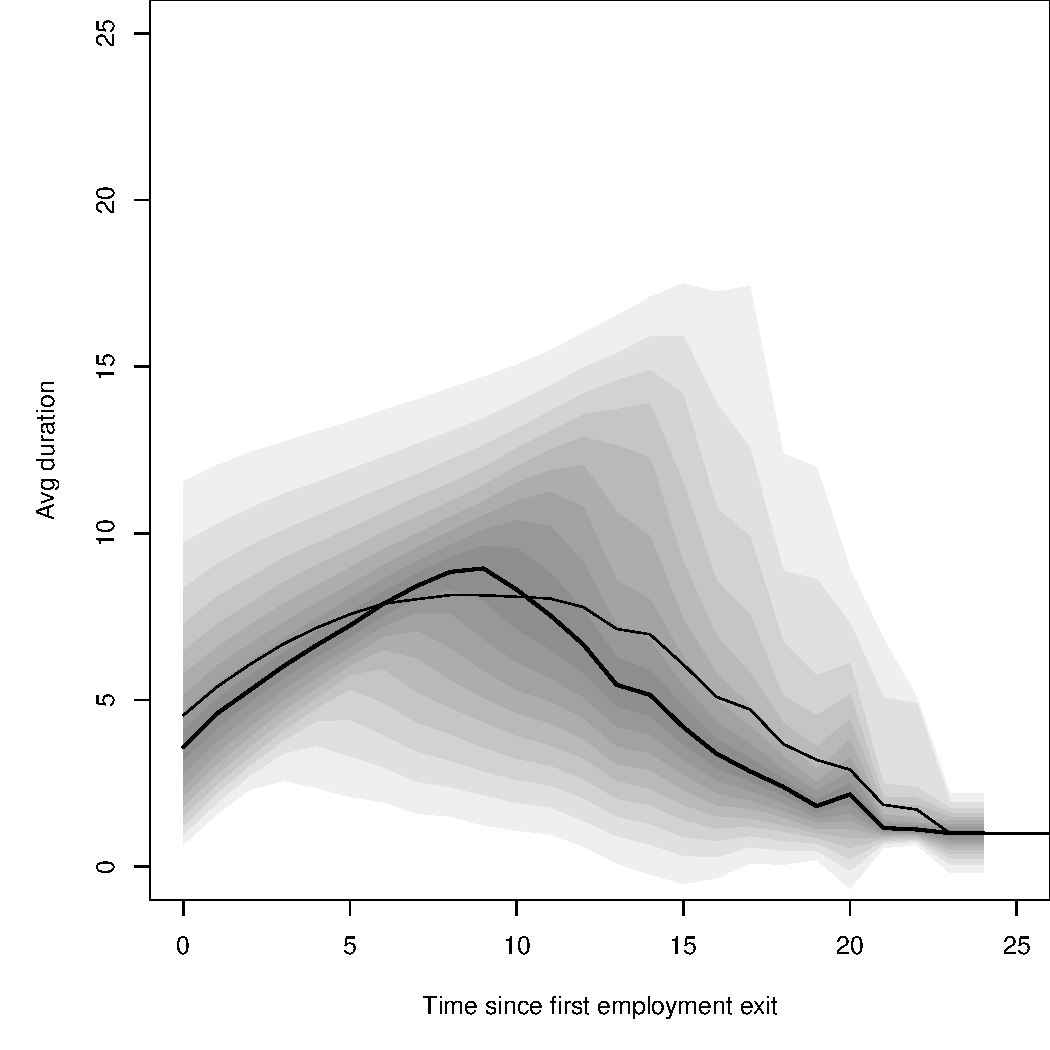
\includegraphics[scale=.4]{Figures/Macro2.pdf}
%\end{subfigure}

%\begin{subfigure}{.49\textwidth}
%\centering
%\caption{Time remaining in spell, mean vs quantiles.}
%\label{fig:macro3}
%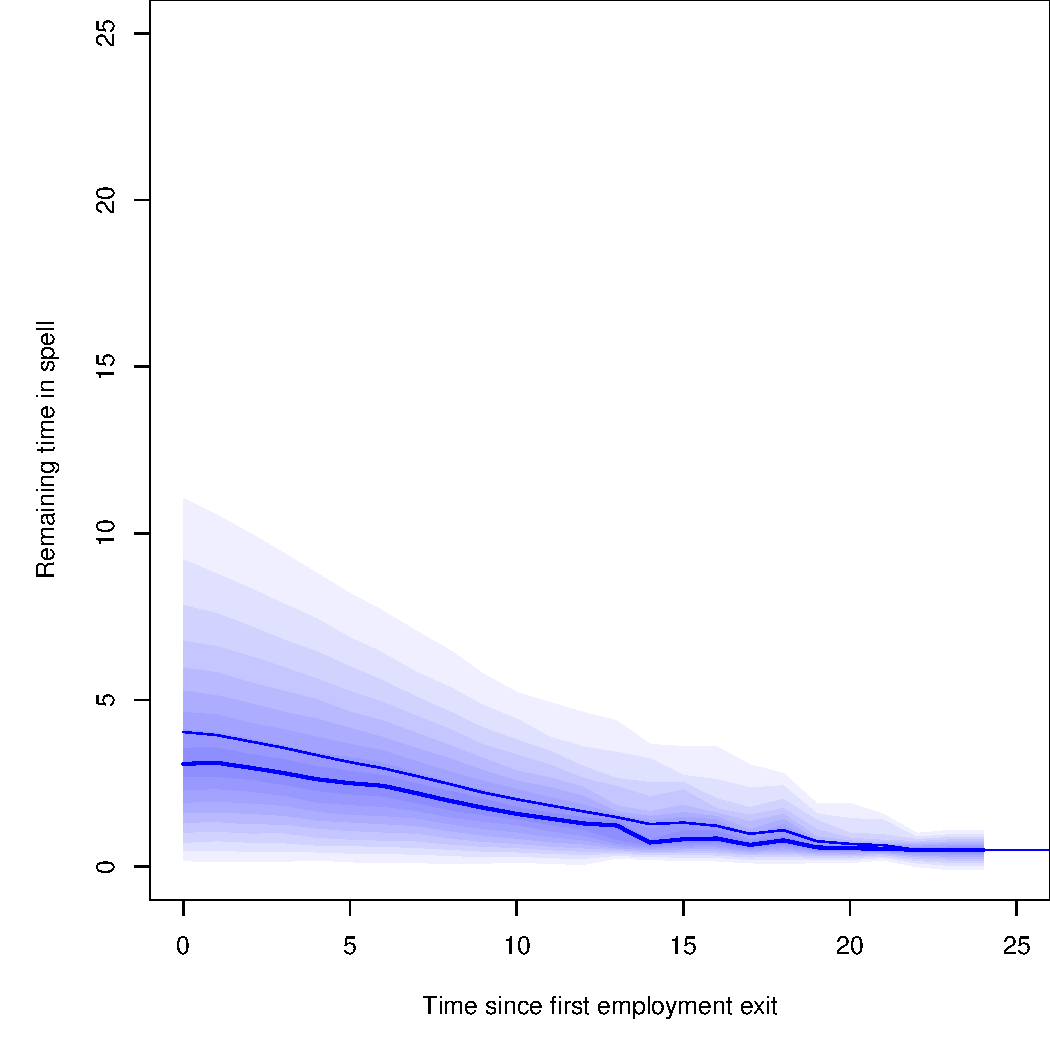
\includegraphics[scale=.4]{Figures/Macro3.pdf}
%\end{subfigure}
%~
%\begin{subfigure}{.49\textwidth}
%\centering
%\caption{Time spent in spell, mean vs quantiles.}
%\label{fig:macro4}
%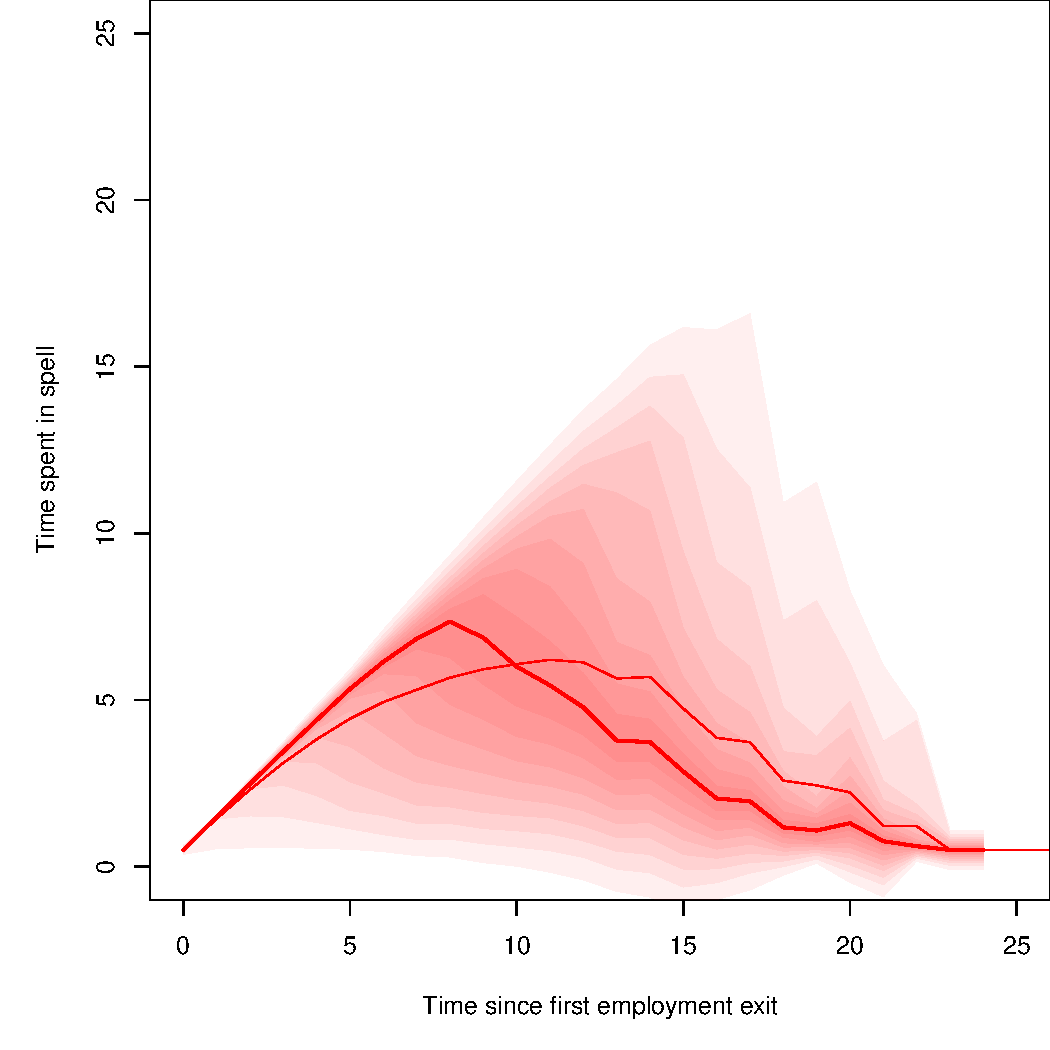
\includegraphics[scale=.4]{Figures/Macro4.pdf}
%\end{subfigure}
%\end{figure}

\subsection{Aggregate patterns}

[A paragraph to say how to aggregate: within structure defined by alignment, aggregate variables defined by clocks]


\section{Applications}

\subsection{Health inequalities}
research questions
\subsubsection{Data}

\subsubsection{Grammatical operations}
Describe the recipes (3)

\subsubsection{Results}
Plots go here and get interpreted

\subsection{Birth interval differentials}

 We use clock and alignment operations to examine the mean time to the second birth over the 15 years following the first birth. We compare these mean times according to the age at first birth (five-year age groups) and the sex of the first child. These comparisons help us answer the question of whether or not the sex of the first child increases the risk (i.e., reduces the mean time) of the second birth. 
 
 In addition, we explore the mean times to the second birth conditional on being a girl and a boy separately. Conditioning on the sex of the second birth allows us to examine, for example, if having a first girl imply a faster next girl, or, if having a first boy imply a faster next boy. All together, these comparisons show how birth interval differential vary substantially by age at first birth and also according to the sex of the first and second child.
 
\subsubsection{Data}

We draw our data from seven waves of the Colombian Demographic and Health Survey (CDHS) collected between 1985 and 2015. The CDHS are nationally representative surveys of women in reproductive ages (15 to 49).

We use full birth histories to reconstruct the reproductive trajectory of all women in the CDHS. We focus on women with at least two children ever born. We show results only for women who had their first birth before age 39 because the proportion of women having their first birth after this age is very small (X\%).

Table \ref{tfert_01} shows the total number of women by groups of age at first birth. According to this table, most of the first births occur between ages 15 and 24.

\begin{table}[ht]
\centering
\begin{tabular}{crrrr}
  \hline
Age at  & \multicolumn{4}{c}{Children ever born} \\ 
first birth & Two & Three & Four+ & Total \\ 
  \hline
10-14 & 616 & 791 & 1754 & 3161 \\ 
  15-19 & 12842 & 10880 & 15001 & 38723 \\ 
  20-24 & 12013 & 7689 & 6476 & 26178 \\ 
  25-29 & 4408 & 1831 & 835 & 7074 \\ 
  30-34 & 1206 & 258 & 50 & 1514 \\ 
  35-39 & 162 & 14 & 4 & 180 \\\hline 
  Total & 31247 & 21463 & 24120 & 76830 \\ 
   \hline
\end{tabular}
\label{tfert_01}
\end{table}

\subsubsection{Grammatical operations}

We use one alignment operation and three different clocks to get at the aggregate-patterns of mean time to second birth. We align women's reproductive trajectory on the age at first birth. For illustrative proposes consider a women interviewed at age 35 who had three children at ages 25, 28 and 33. The first two were girls and the last one a boy. The following table represents her reproductive trajectory.

\begin{center}
\begin{tabular}{c|ccccccccccccc}
\hline
    Age & 15 & $...$ & 25 & 26 & 27 & 28 & 29 & 30 & 31 & 32 & 33 & 34 & 35 \\
    Sex & - & $...$ & girl & - & - & girl & - & - & - & - & boy & - & - \\\hline
\end{tabular}
\end{center}

The first clock counts the number of years to the second birth. Following the previous example, the aligned-clocked sub-sequence for ages 25 to 28 will look like this: 3-2-1-0. This sub-sequence means that when the first birth occur (at age 25) this women had three years left, before the second birth. At age 26, she had two years left, etc. By age 28, she had a second birth, for which the clock equals zero.

We define two analogous clocks to examine differences by the sex of the second birth. In the first case, the clock counts the remaining years to the next boy. In the second case, the clock counts the remaining years to the next girls. If a woman did not have a boy or a gilt, the clock does....(what does it do?). Table X displays the aligned sequence, starting at time zero (age at first birth, and the three clocks that input time into women's reproductive trajectory.

\begin{center}
\begin{tabular}{l|ccccccccccc}
\hline
    Time since birth & 0 & 1 & 2 & 3 & 4 & 5 & 6 & 7 & 8 & 9 & 10 \\
    Age & 25 & 26 & 27 & 28 & 29 & 30 & 31 & 32 & 33 & 34 & 35 \\
    Sex & girl & - & - & girl & - & - & - & - & boy & - & - \\
    %\multicolumn{11}{l}{\textbf{Clocks}}\\
    Clock: To second birth & 3 & 2 & 1 & 0 & - & - & - & - & - & - & - \\
    Clock: To next boy & 8 & 7 & 6 & 5 & 4 & 3 & 2 & 1 & 0 & - & - \\
    Clock: To next girl & 3 & 2 & 1 & 0 & - & - & - & - & - & - & - \\\hline
\end{tabular}
\end{center}

Note the information that is ignore AND the coincidence between the to clocks.

Once this alignment operation is performed and the three clocks are computed for all women in the sample, we take the mean of the columns. These means should be interpreted as conditional mean time to second birth, to next boy, and next girl.

\subsubsection{Results}
Figure \ref{fert_01} displays the aggregated patterns of the mean time to the second birth over the 10 years after the first child by women's age at first birth, and according to the sex of the first child. Overall, the mean time to second births range between 0.5 and slightly more than 3 years. There are significant difference across age at first birth groups

\begin{figure}[H]
    \centering
    \caption{Mean time to second birth by age at first birth (five-year age groups) and sex of the first child. Colombian DHS 1985-2015}
    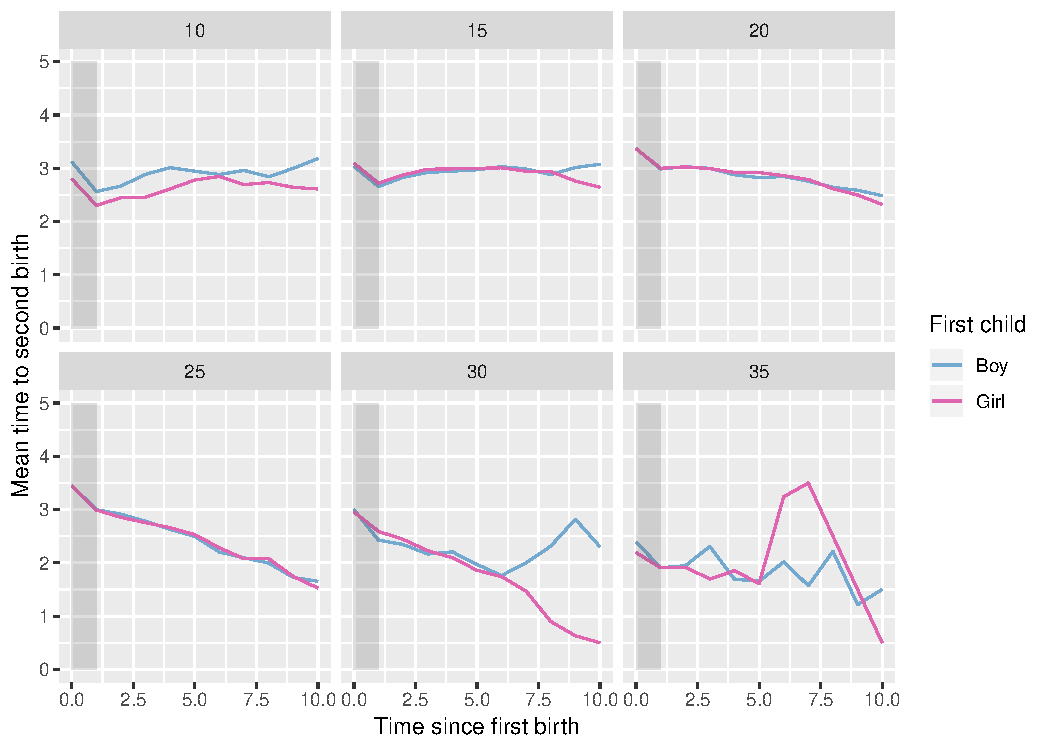
\includegraphics{Spells/Figures/mt_second_birth_by_sex_first.pdf}
    \label{fert_01}
    Note: the gray rectangle of one year width indicate the birth of twins, i.e., mean time to next birth less than one year.
\end{figure}

Among the first three age at first birth groups, the mean time to second birth is relatively flat over the 10 years following the first birth meaning that for women who had their first birth between ages 10 and 19 (and moved on to have at least one more), the risk of a second birth is constant over the period after the first child. On average, between 2.5 and 3 years precede the birth of a second child. Additionally, in the first age group, the birth of a boy is associated with higher mean time to second birth during the 10 years after the first birth.

Among the other three age at first birth groups, the mean time to second birth decline over time. This decline is specially marked among the last two groups which is consistent with the limit of the reproductive period for women. In these three groups, difference by sex of the first birth are very small, however in the 25-29 age group these small differences are consistent over the ten-year period after the first birth, which suggests they may be important when aggregated. Finally, erratic patterns in the last age groups may be due to small sample size, i.e., very few women having their first child after age 35.

Figure \ref{fert_02} examine the mean time to next boy, i.e., the mean number of years that precede a male birth, again, by women's age at first birth and the sex of the first child. Because of the way clock are defined, the mean time to next boy are about twice the mean time to second birth (refer to Figure \ref{fert_01}. Overall, right after the first birth, the mean number of year that precede a male birth among women who eventually had it is between five and 7.5 years.

\begin{figure}[H]
    \centering
    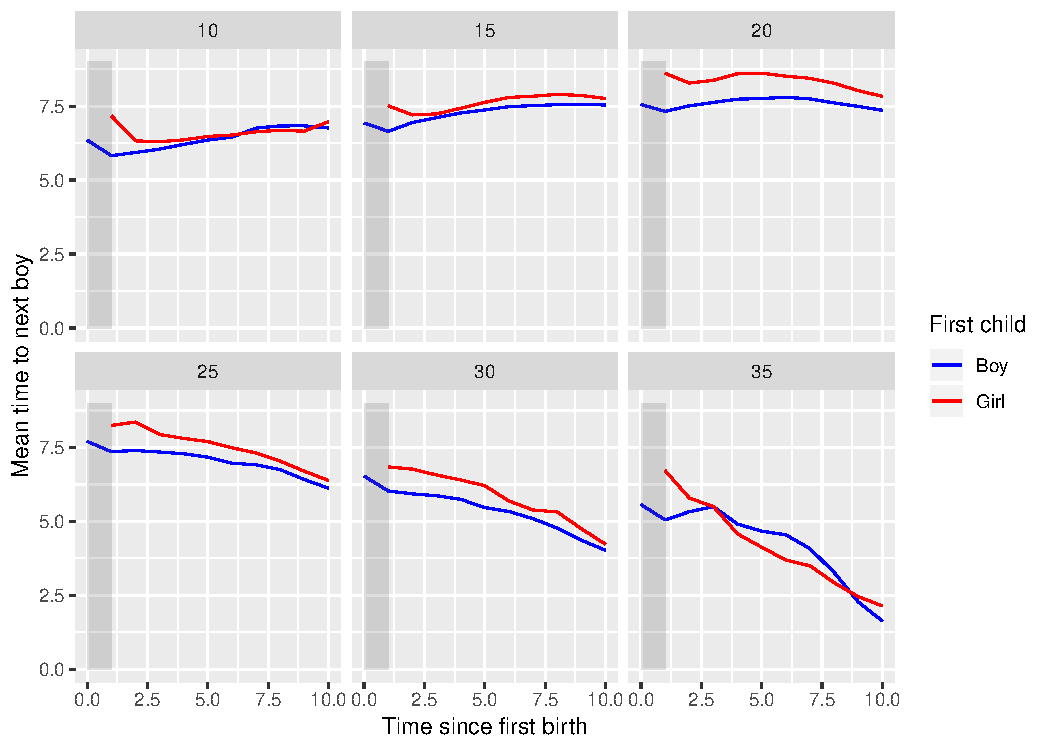
\includegraphics{Spells/Figures/mt_second_boy_by_sex_first.pdf}
    \caption{Caption}
    \label{fert_02}
\end{figure}

In addition, figure \ref{fert_02} shows that, between ages 15 and 34, having a male first birth is associated with a faster transition to a second male birth regardless. These are the ages where fertility is concentrated for which this association is robust. Consistently with the definitions of the clocks, the sex gap widens a little over time, as eventual female births give higher values to the clock that counts the time to next boy, and narrows towards the en of the ten-year period, because male birth finally occur. 

A similar pattern is observed in Figure \ref{fert_03} for the mean time to next girl. On average, between five and 7.5 years precede the birth of a girl after the birth of a first child. Female births are associated with a faster transition to a female birth

\begin{figure}[H]
    \centering
    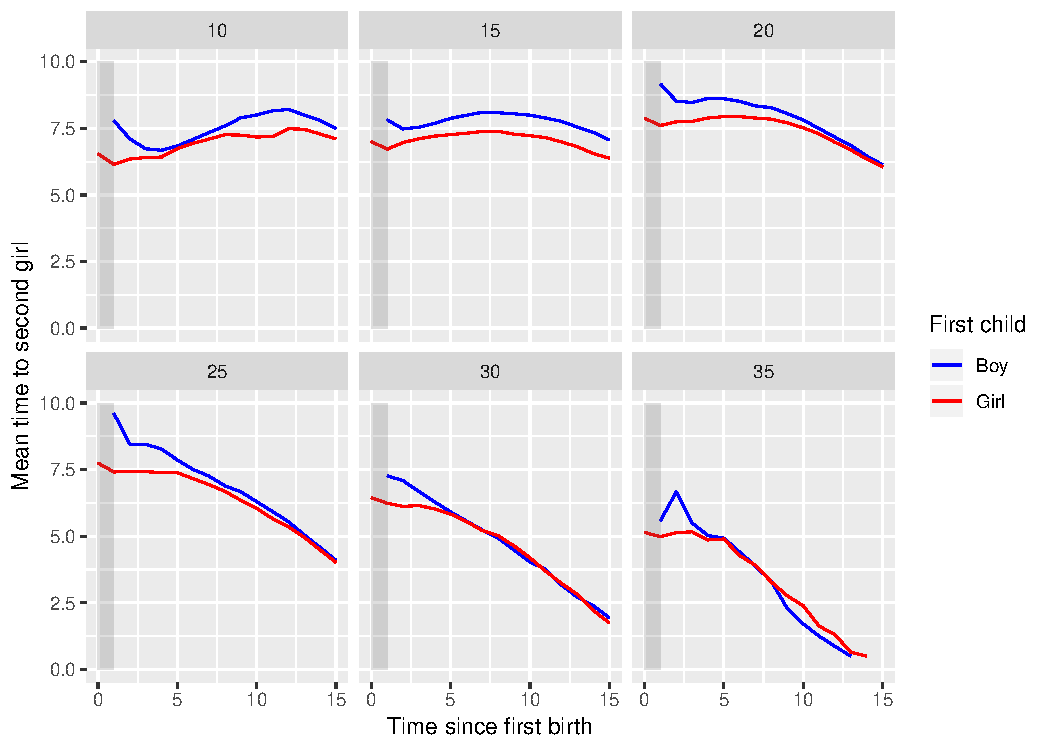
\includegraphics{Spells/Figures/mt_second_gir_by_sex_first.pdf}
    \caption{Caption}
    \label{fert_03}
\end{figure}

Compared to the mean time to the next boy, the mean time to next girl displays larger differences by sex of the first child. In other words, the positive association between the sex of the first birth and the mean time of a birth of the same sex, is stronger for girl than boys.

Righ censoring issues...

\section{Discussion}

We propose a grammar of data operations to allow for creative derivation of demographic macro patterns. Our examples makeup a small subset of those possible, even with the small state space used in our example. To give a sense of the number of macro patterns possible, multiply (1) the number of state categories, (2) episode selection options (first, last, longest, etc), (3) alignment options (left, right, center, etc), and clock options (duration, time spent/left, order, and many others), and it becomes evident that we might have produced over one hundred different macro patterns, just for this relatively simple example case. 

It may be surprising to notice that most of these patterns, even though ours resulted from a simple Markov process with a small set of simple and monotonic age patterns, have some character to them. They contain information. Presumably the age patterns that entered into said Markov model do not capture the entire story, and raw observed state sequences are expected to bear stronger degrees of co-dependency. And if we wish to learn something new about a given demographic process, the researcher has (i) large degrees of freedom in selecting macro episode patterns, and (ii) is limited only by one's own creativity in doing so. 

The purpose of episode clocks and sequence realignment is to detect important patterns in data (or model results) that are likely to otherwise go unnoticed. Some reasonable priors might include that (i) life course events condition each other; (ii) temporal proximity to life course transitions is likely to be an important predictor of other transitions; (iii) within-episode patterns of other characteristics might be monotonically increasing or decreasing, concave, or convex. Aggregate patterns derived after such operations may be sharper and of more obvious interpretation and consequence than are age patterns. 

\section*{Promises}
This manuscript is an early draft. In a future version we will offer vignette-style applications for a selection of different demographic phenomena, including health and fertility/family demography, resident status of migrants, each with a variety of programmatically generated macro patterns. 

\section*{Acknowledgements}
This work has benefitted from discussions with Christian Dudel, Erik Vickstrom, Marcus Ebeling, Jutta Gampe, and Maarten Bijlsma. Indeed, some may even become coauthors as this work progresses.

\FloatBarrier
\singlespacing
\bibliographystyle{plainnat}
  \bibliography{references} 
\end{document}
